\documentclass[12pt,dvipdfm]{beamer}

\usepackage{hcystyle}

%%%%%%%文档正文
\begin{document}

%标题作者等信息。
%这些信息将自动生成ppt的第一页
\title[毕业设计答辩]{\LARGE{毕业设计答辩\\}}
%\subtitle{基于动态链接技术的{\cp web}服务器动态扩展功能\\接口的设计与实现}
\author[黄丛宇]{黄丛宇\\06161032\\指导老师:马瑞芳}
\institute[西安交通大学 软件学院]{西安交通大学 软件学院 软件62班}
\date{\today}

\begin{frame}	
	\titlepage
\end{frame}

\begin{frame}
	\frametitle{目录}
	\tableofcontents
\end{frame}

\section{课题名称}
%第二页
\begin{frame}
	\frametitle{课题名称}
	
	\begin{center}
	{\Large
			基于动态链接技术的web服务器动态扩展功能\\
				接口的设计与实现
	}
	\end{center}
\end{frame}

\section{背景和意义}
\begin{frame}
	\frametitle{背景和意义}
	\begin{itemize}
		\item Web服务器:
			\begin{itemize}
				\item[-] 互联网的核心组成部分,支撑整个互联网应用服务。
				\item[-] 适应互联网应用的不断更新变化。
				\item[-] 必须保证7*24小时的运行。
			\end{itemize}
		\pause
		\item {\cp Web}服务器现状:
			\begin{itemize}
				\item[-] 大部分都不支持功能的动态增加。
				\item[-] 必须重启或重新编译。
			\end{itemize}
	\end{itemize}
\end{frame}

\begin{frame}
	\frametitle{背景和意义}
	\begin{itemize}
		\item 针对以上问题,本课题将基于动态链接库技术,使服务器在运行期间,可以动态的获知模块的增加并加载模块。
		\pause
		\item 本系统实现了服务器的基本功能,重点实现模块动态加载特性。
	\end{itemize}
\end{frame}

\section{HTTP协议分析}

\begin{frame}
	\frametitle{test}
\end{frame}

\begin{frame}
	\frametitle{HTTP协议简介}
	
HTTP协议(Hypertext Transfer Protocol,超文本传输协议)是一个属于应用层的面向对象的协议。它于1990年提出。主要用于从WWW服务器传输超文本到本地浏览器的传送协议。

HTTP协议具有如下特点:
\five{
	\begin{enumerate}
		\item 支持客户/服务器模式。
		\item 简单快速:客户向服务器请求服务时,只需传送请求方法和路径。
		\item 灵活:HTTP允许传输任意类型的数据对象。
		\item 无连接:无连接的含义是限制每次连接只处理一个请求。
		\item 无状态:协议对于事务处理没有记忆能力。
	\end{enumerate}
}
\end{frame}

\begin{frame}
	\frametitle{HTTP协议处理过程}
	\begin{figure}[htbp]
	\centering
	\caption{HTTP协议处理过程}
	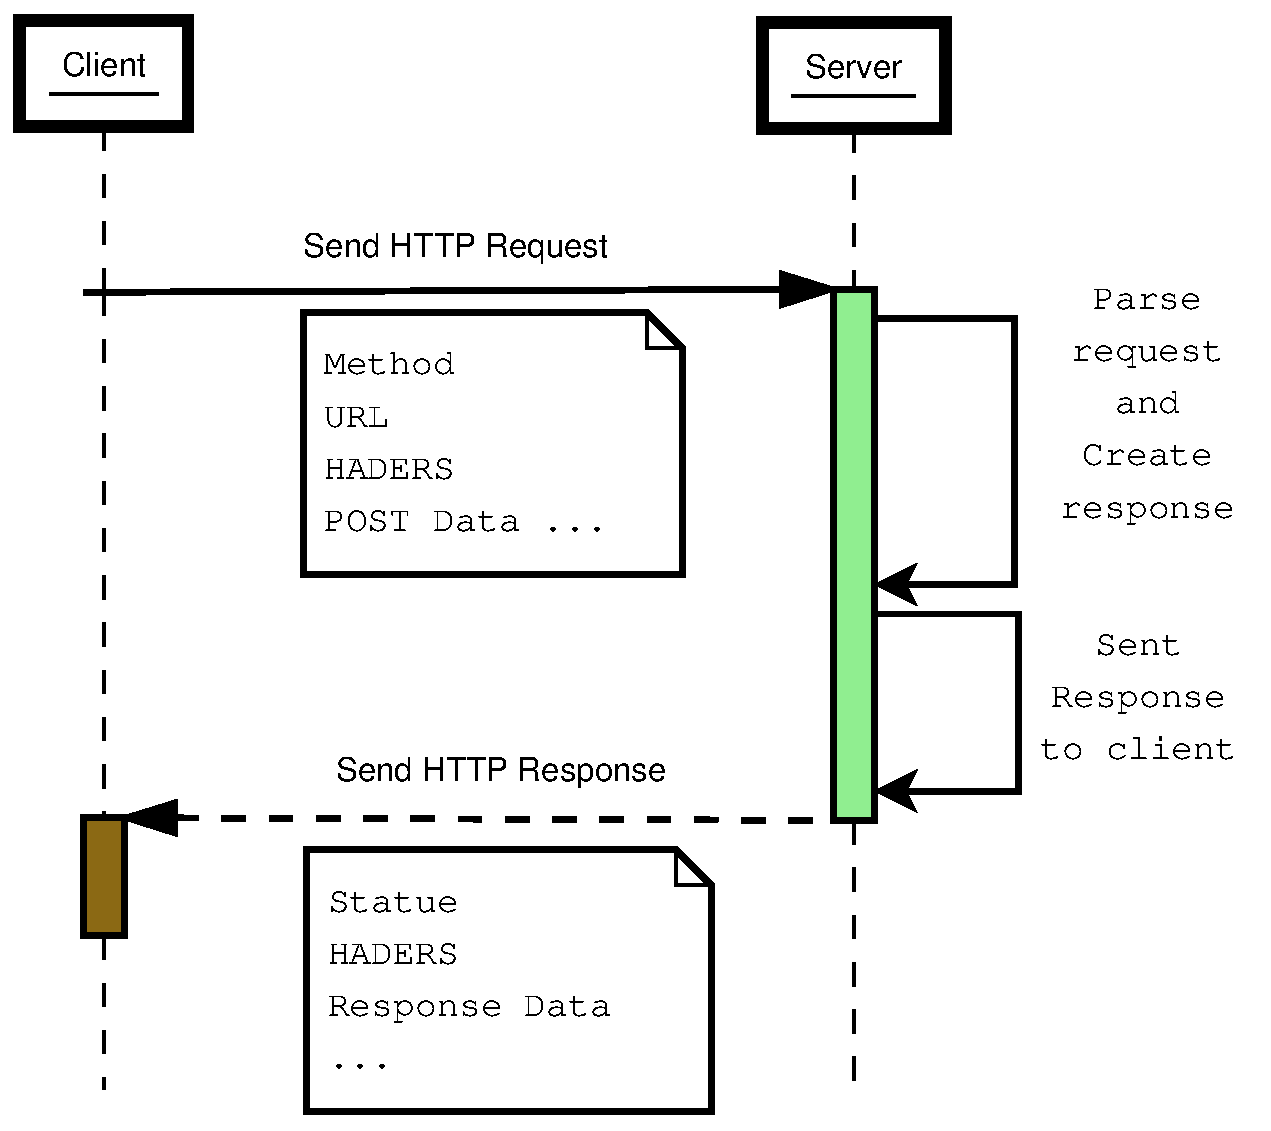
\includegraphics[height=6cm, width=7cm]{http.eps}
	\end{figure}
\end{frame}

\begin{frame}
	\frametitle{HTTP协议格式}
\end{frame}

\begin{frame}
	\frametitle{需要处理的HEADERS}
\end{frame}

\section{接口设计}
\section{服务器设计}
\section{接口实现}
\section{服务器实现}
\section{运行结果}

\begin{frame}
	\frametitle{结束}
	\begin{center}
	{\Huge
		\textsl{That's all!}
	}
	\end{center}
\end{frame}

\end{document}
